% -*- mode: noweb; noweb-default-code-mode: R-mode; -*-
\documentclass[a4paper]{article}

\title{A Test File}
\author{Friedrich Leisch}


\usepackage{a4wide}

\usepackage{/usr/share/R/share/texmf/Sweave}
\begin{document}

\maketitle

A simple example that will run in any S engine: The integers from 1 to
10 are
\begin{Verbatim}
 [1]  1  2  3  4  5  6  7  8  9 10
\end{Verbatim}

We can also emulate a simple calculator:
\begin{Schunk}
\begin{Sinput}
> 1 + 1
\end{Sinput}
\begin{Soutput}
[1] 2
\end{Soutput}
\begin{Sinput}
> 1 + pi
\end{Sinput}
\begin{Soutput}
[1] 4.141593
\end{Soutput}
\begin{Sinput}
> sin(pi/2)
\end{Sinput}
\begin{Soutput}
[1] 1
\end{Soutput}
\end{Schunk}

Now we look at Gaussian data:

\begin{Schunk}
\begin{Soutput}
 [1]  1.975020082 -0.596560482  0.379859890  1.279714455 -0.305434367
 [6]  0.001238350 -0.434984359 -0.316102851 -0.050375397  0.541407408
[11] -0.559675652 -0.269072911  1.352853069 -1.826236281 -0.021364586
[16]  0.201180022  0.744513870  1.080508219  0.524392703  0.226922429
\end{Soutput}
\begin{Soutput}
	One Sample t-test

data:  x 
t = 1.0387, df = 19, p-value = 0.312
alternative hypothesis: true mean is not equal to 0 
95 percent confidence interval:
 -0.1993585  0.5921388 
sample estimates:
mean of x 
0.1963902 
\end{Soutput}
\end{Schunk}
Note that we can easily integrate some numbers into standard text: The
third element of vector \texttt{x} is 0.379859889601437, the
$p$-value of the test is 0.312. % $

Now we look at a summary of the famous iris data set, and we want to
see the commands in the code chunks:



% the following code is R-specific, as data(iris) will not run in Splus. 
% Hence, we mark it as R code. 
\begin{Schunk}
\begin{Sinput}
> data(iris)
> summary(iris)
\end{Sinput}
\begin{Soutput}
  Sepal.Length    Sepal.Width     Petal.Length    Petal.Width   
 Min.   :4.300   Min.   :2.000   Min.   :1.000   Min.   :0.100  
 1st Qu.:5.100   1st Qu.:2.800   1st Qu.:1.600   1st Qu.:0.300  
 Median :5.800   Median :3.000   Median :4.350   Median :1.300  
 Mean   :5.843   Mean   :3.057   Mean   :3.758   Mean   :1.199  
 3rd Qu.:6.400   3rd Qu.:3.300   3rd Qu.:5.100   3rd Qu.:1.800  
 Max.   :7.900   Max.   :4.400   Max.   :6.900   Max.   :2.500  
       Species  
 setosa    :50  
 versicolor:50  
 virginica :50  
\end{Soutput}
\end{Schunk}


\begin{figure}[htbp]
  \begin{center}
\begin{Schunk}
\begin{Sinput}
> library(graphics)
> pairs(iris)
\end{Sinput}
\end{Schunk}
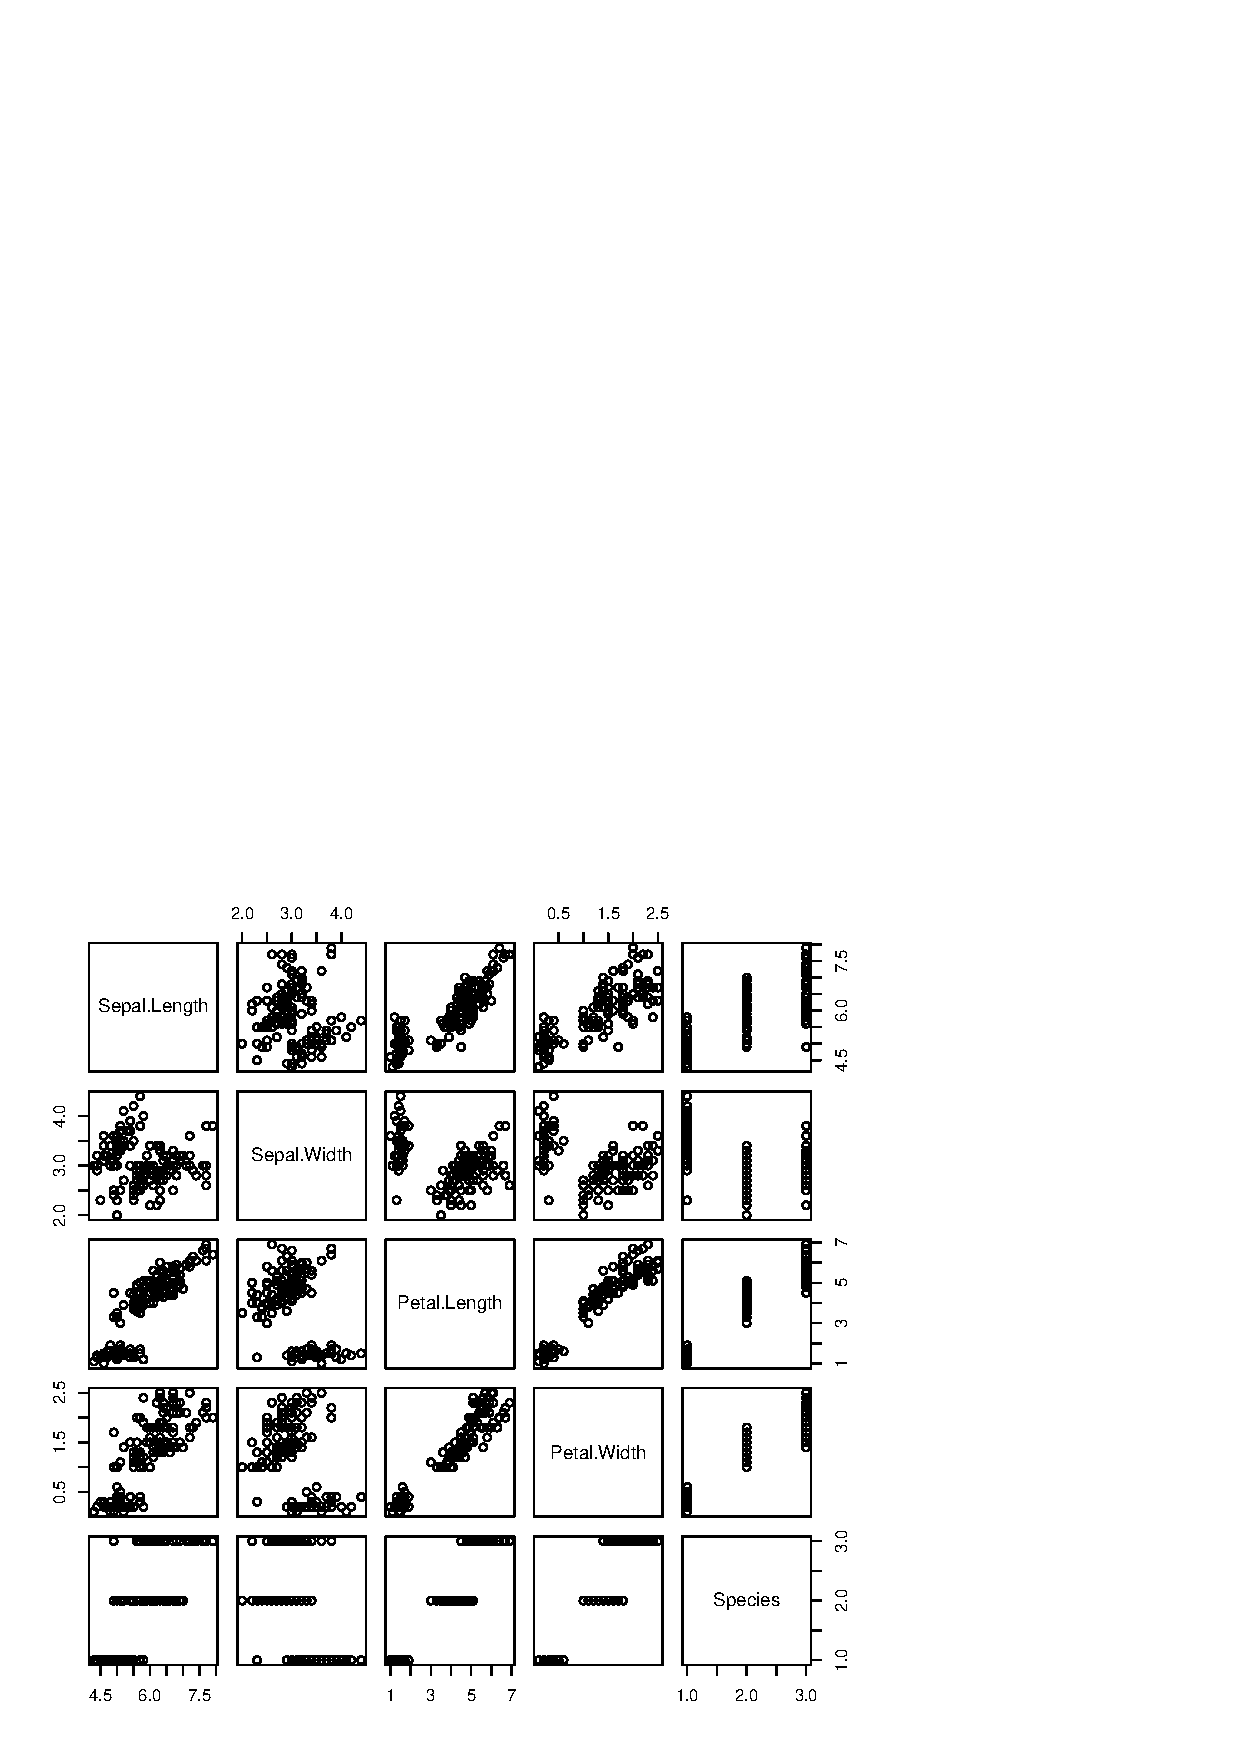
\includegraphics{Sweave-test-1-006}
    \caption{Pairs plot of the iris data.}
  \end{center}
\end{figure}

\begin{figure}[htbp]
  \begin{center}
\begin{Schunk}
\begin{Sinput}
> boxplot(Sepal.Length ~ Species, data = iris)
\end{Sinput}
\end{Schunk}
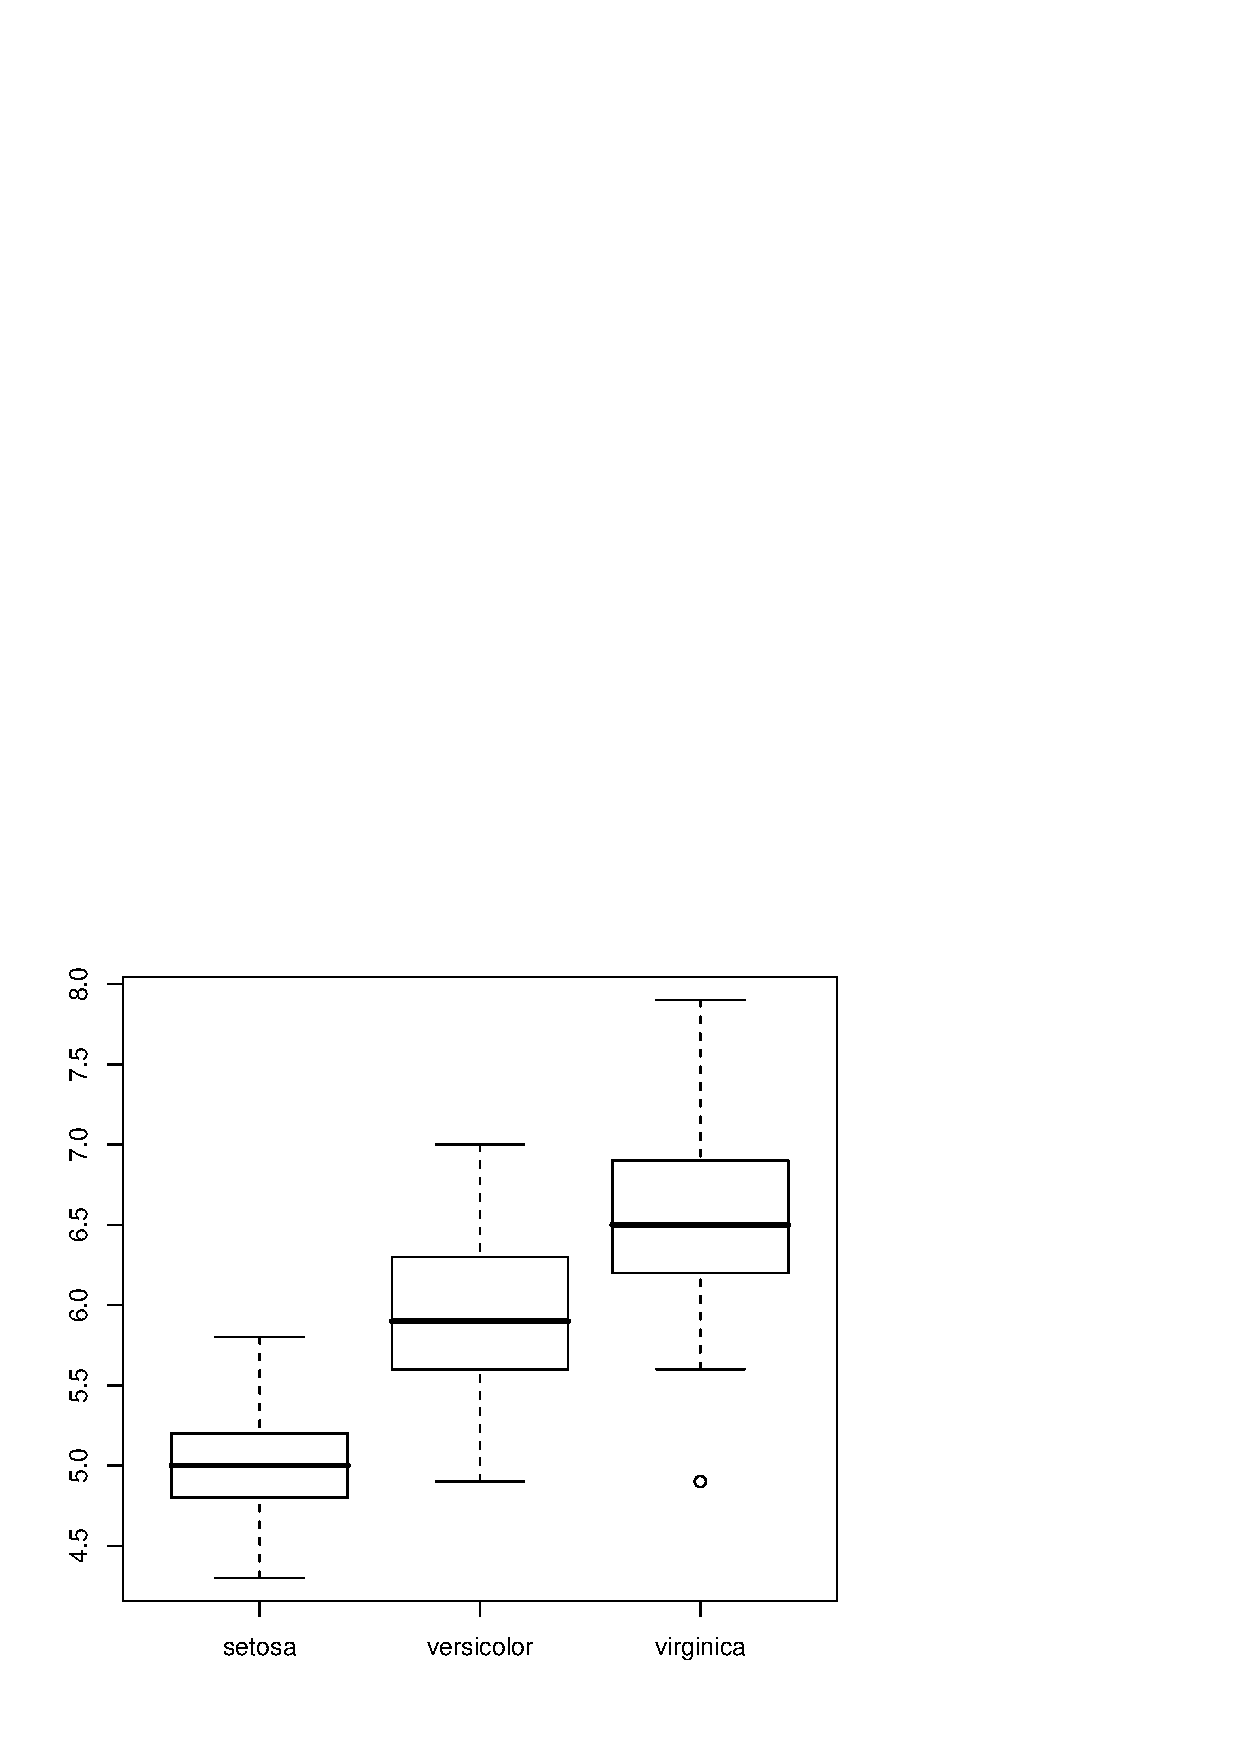
\includegraphics{Sweave-test-1-007}
    \caption{Boxplot of sepal length grouped by species.}
  \end{center}
\end{figure}


% R is not S-PLUS, hence this chunk will be ignored:

\end{document}


